\section{計測手法}
\subsection{ストレッチセンサ計測アルゴリズム}
\ref{sec:RC回路}にて示す通り,ストレッチセンサの静電容量変化の計測にはRC回路を用いた時定数の計測で行った.
なお,この時定数の計測にはNucleoF303K8といったマイコン評価ボードを使用した.また,それらのコードの記述にはmbedライブラリを使用した.
使用したソースコードは下記リンクにて公開している.計測アルゴリズムはFig.\ref{fig:algorithm}にて示すように
1000Hzで計測を実行し,100Hzごとに計測データの平均値をSerial通信を用いてPCに出力した.
また,2000Hzで出力ピンの状態を切り替え,ストレッチセンサに電荷が残らないようにした.

ソースコード:https://os.mbed.com/users/HidetoN/code/Cap-Sensor/

\begin{figure}[h]
    \begin{center}
     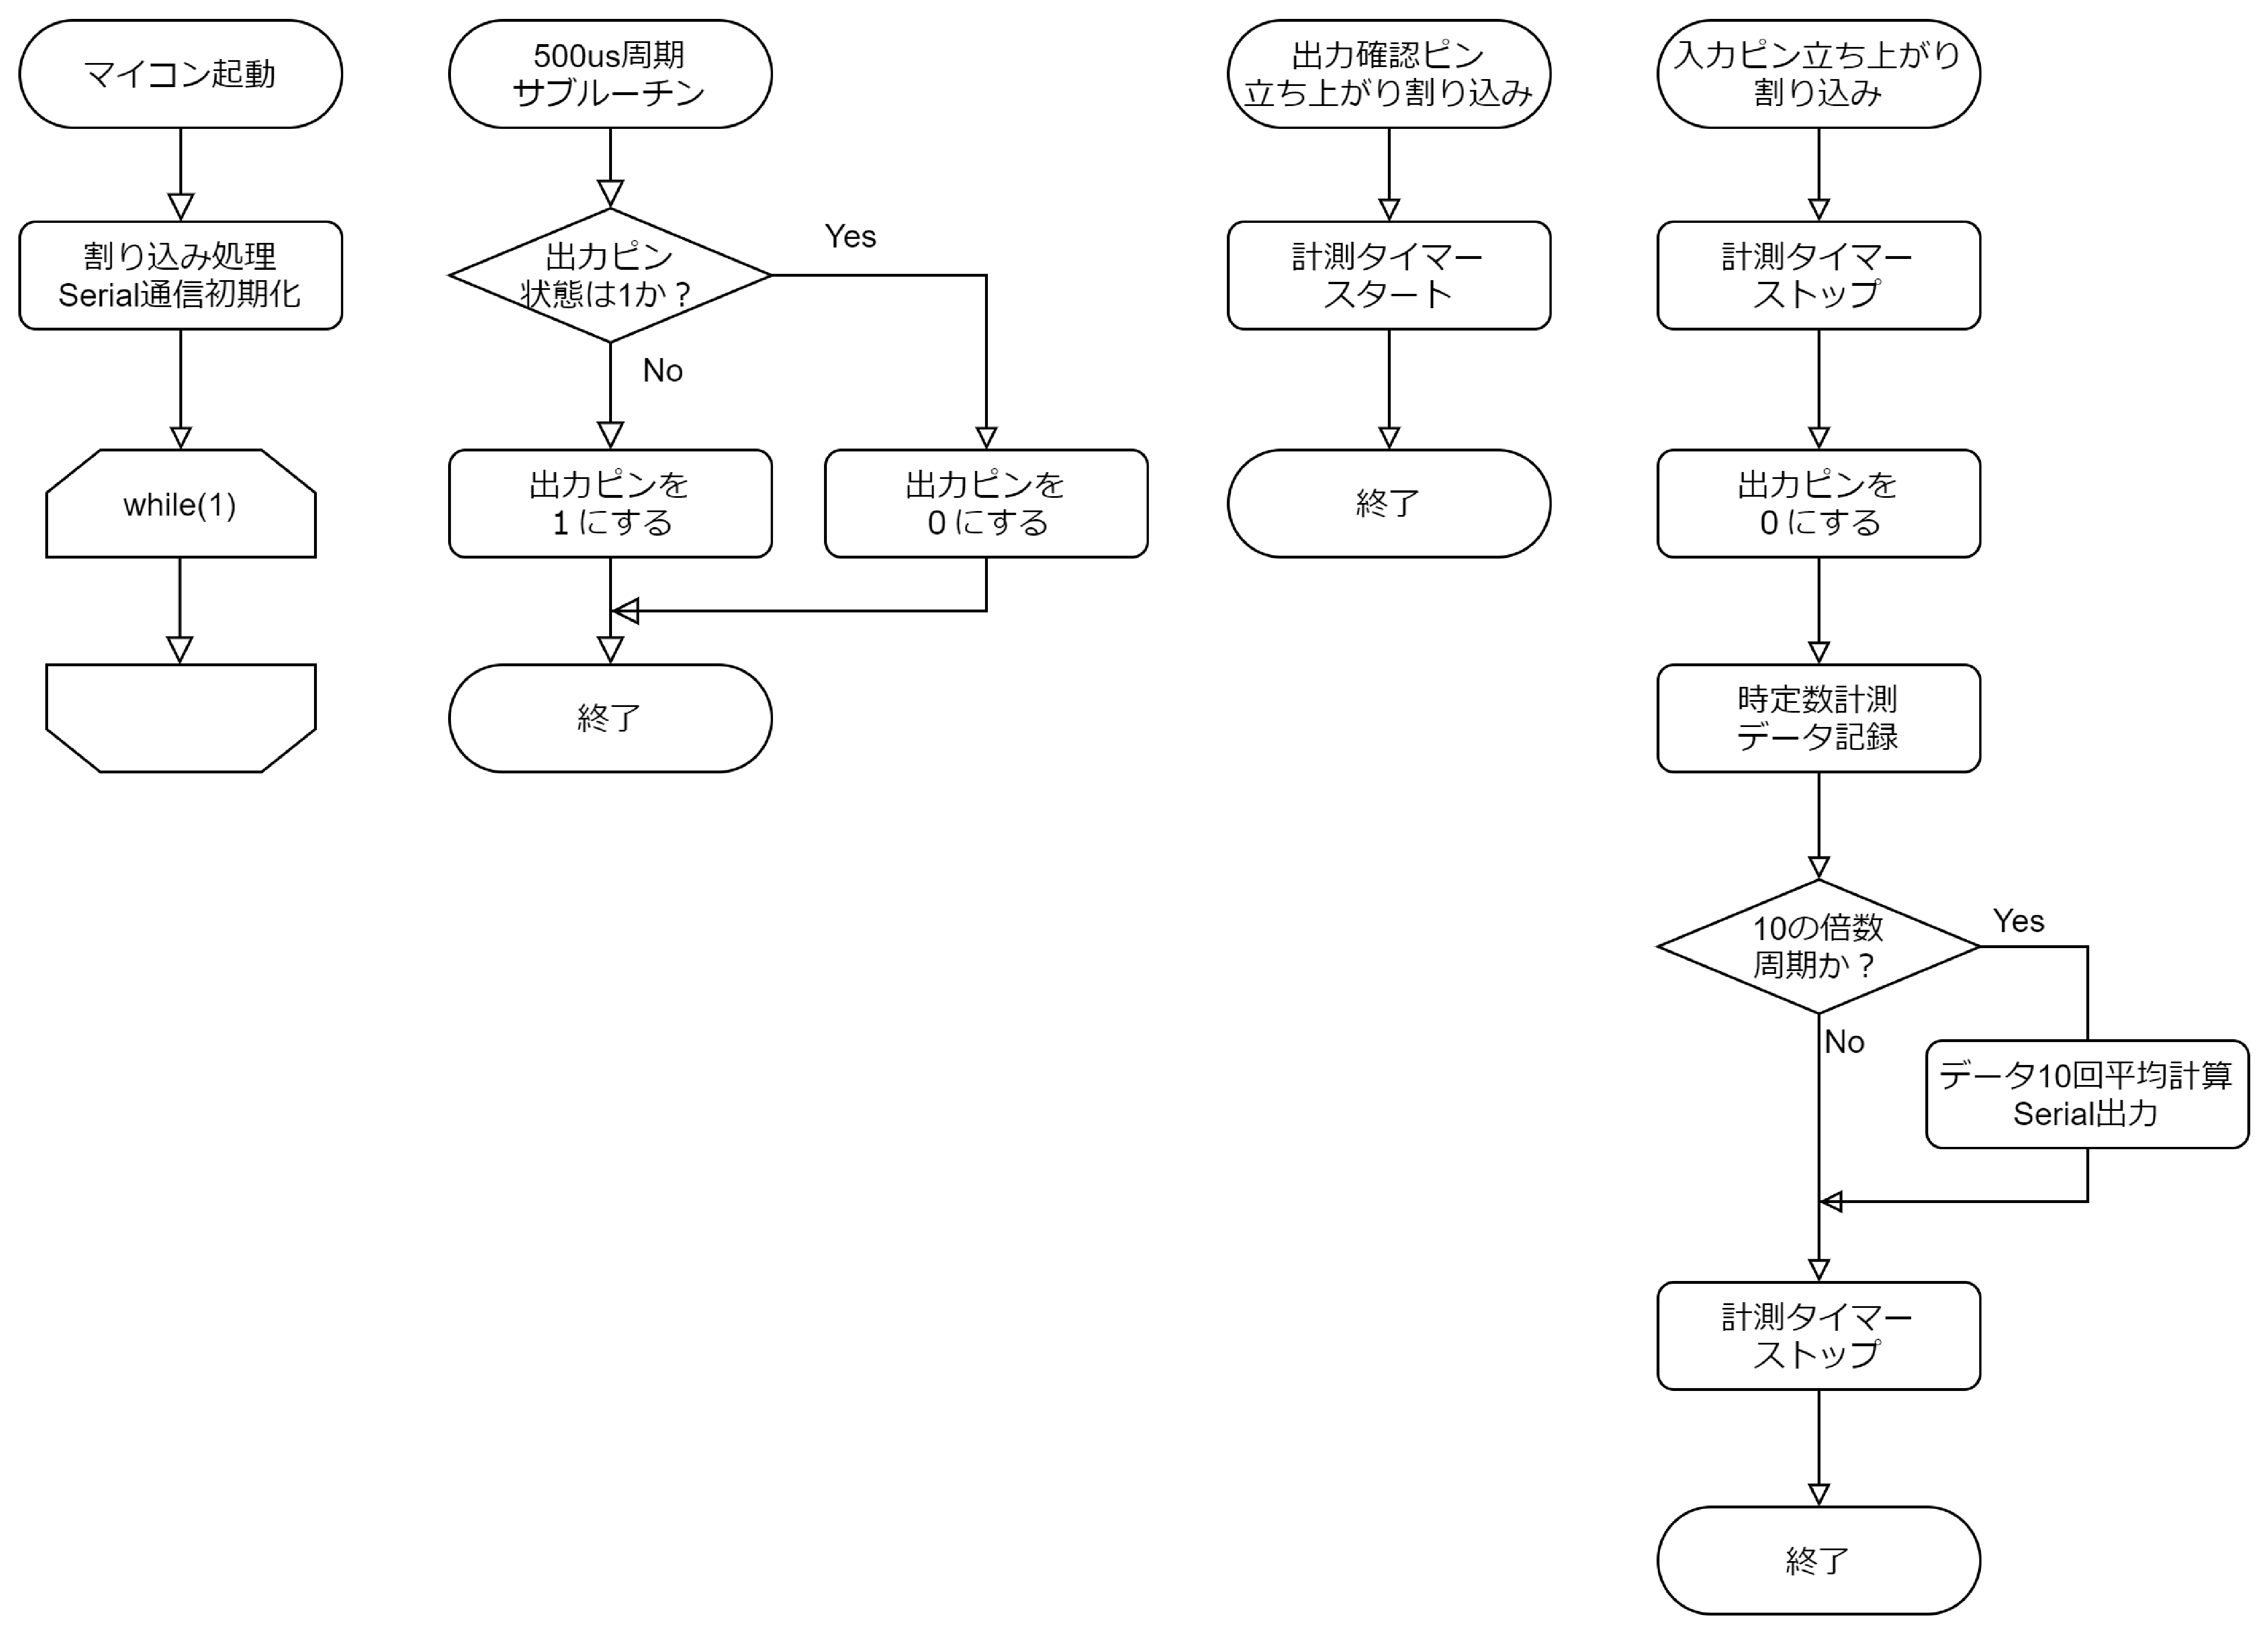
\includegraphics[width=0.9\columnwidth,clip]{./3_analysis/algorithm.eps}
     \caption{計測プログラムにおけるアルゴリズム}
     \label{fig:algorithm}
    \end{center}
\end{figure}

\subsection{ストレッチセンサ計測システム}
ストレッチセンサの計測データはNucleoF303K8よりSerial通信によって921600bpsで出力される.
制御アルゴリズムの部分でも示したが,1000Hz周期で取得したデータの平均値が100Hz周期に出力される.
このデータをTeraTermのログ取得機能を用いてcsvファイルとして保存した.
なお,足関節ロボット制御用PCの処理の都合上,別PCを用いて結果の取得を行った.
\begin{figure}[h]
    \begin{center}
        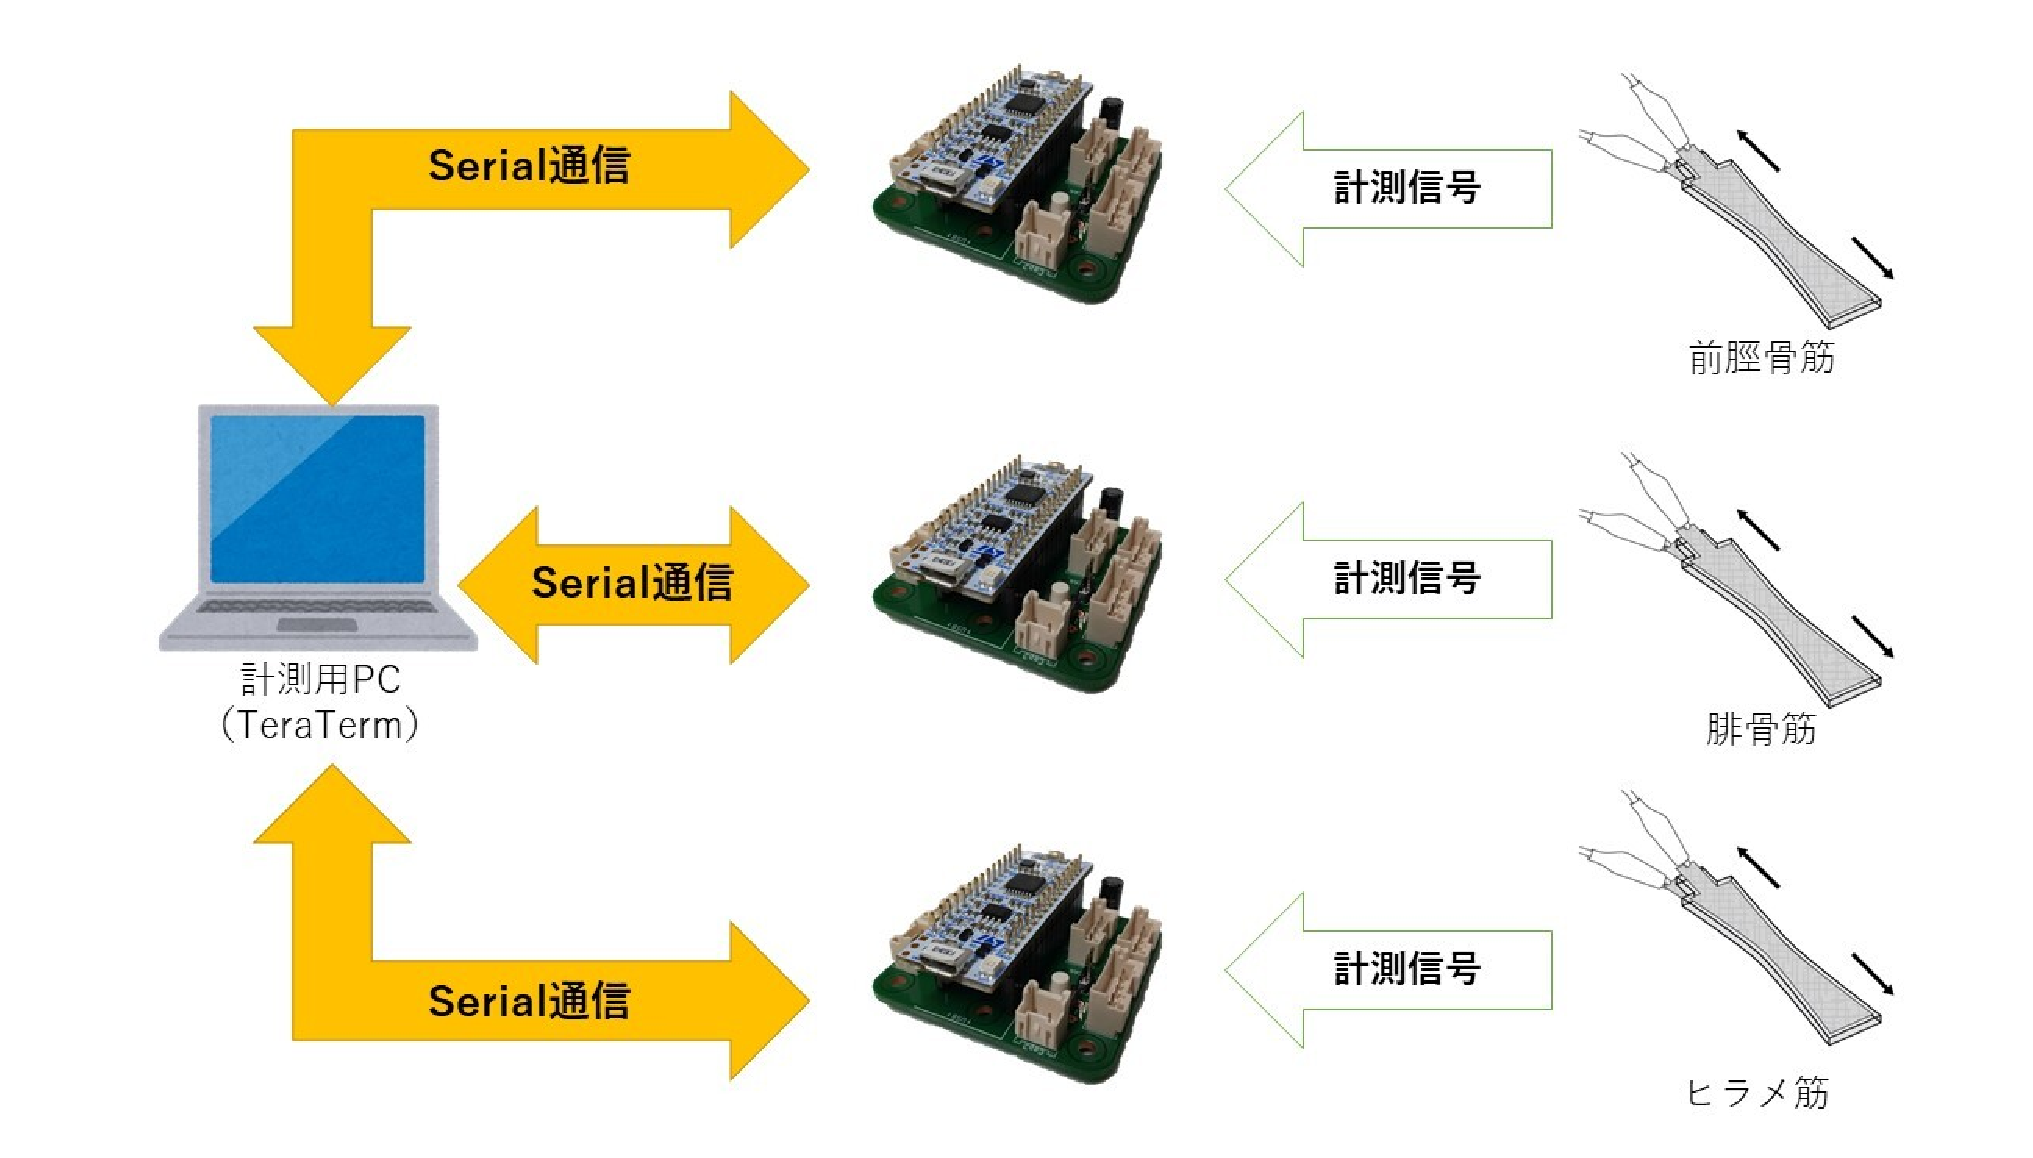
\includegraphics[width=0.78\columnwidth,clip]{./3_analysis/getSystem.eps}
        \caption{計測システム概略図}
        \label{getSystem}
    \end{center}
\end{figure}

\subsection{足関節ロボット駆動システム}
足関節ロボットの駆動システムには従来から存在するペダリングロボット,2足歩行ロボットのシステムと同様のシステムを利用した.
以下にそのシステムに関して記述する.

まず,Fig.\ref{fig:compressor}にて示す,エアーコンプレッサーで8気圧まで圧縮空気を作成し,気圧調整弁を用いて6気圧まで減圧を行った.
続いて,制御用PCに搭載されたDAボードより,空気圧制御盤にアナログ信号を送信する.なお,この電圧指令は550段階で制御が行うことが出来る.
この電圧指令を元に空気圧制御盤に搭載された空気圧制御器によって可変的に空気圧の制御を各人工筋に対して行う.

\newpage

\begin{figure}[h]
    \begin{center}
     
\includegraphics[width=0.65\columnwidth,clip]{./3_analysis/compressor.eps}
     \caption{使用したエアーコンプレッサー}
     \label{fig:compressor}
    \end{center}
\end{figure}

\begin{figure}[h]
    \begin{center}
     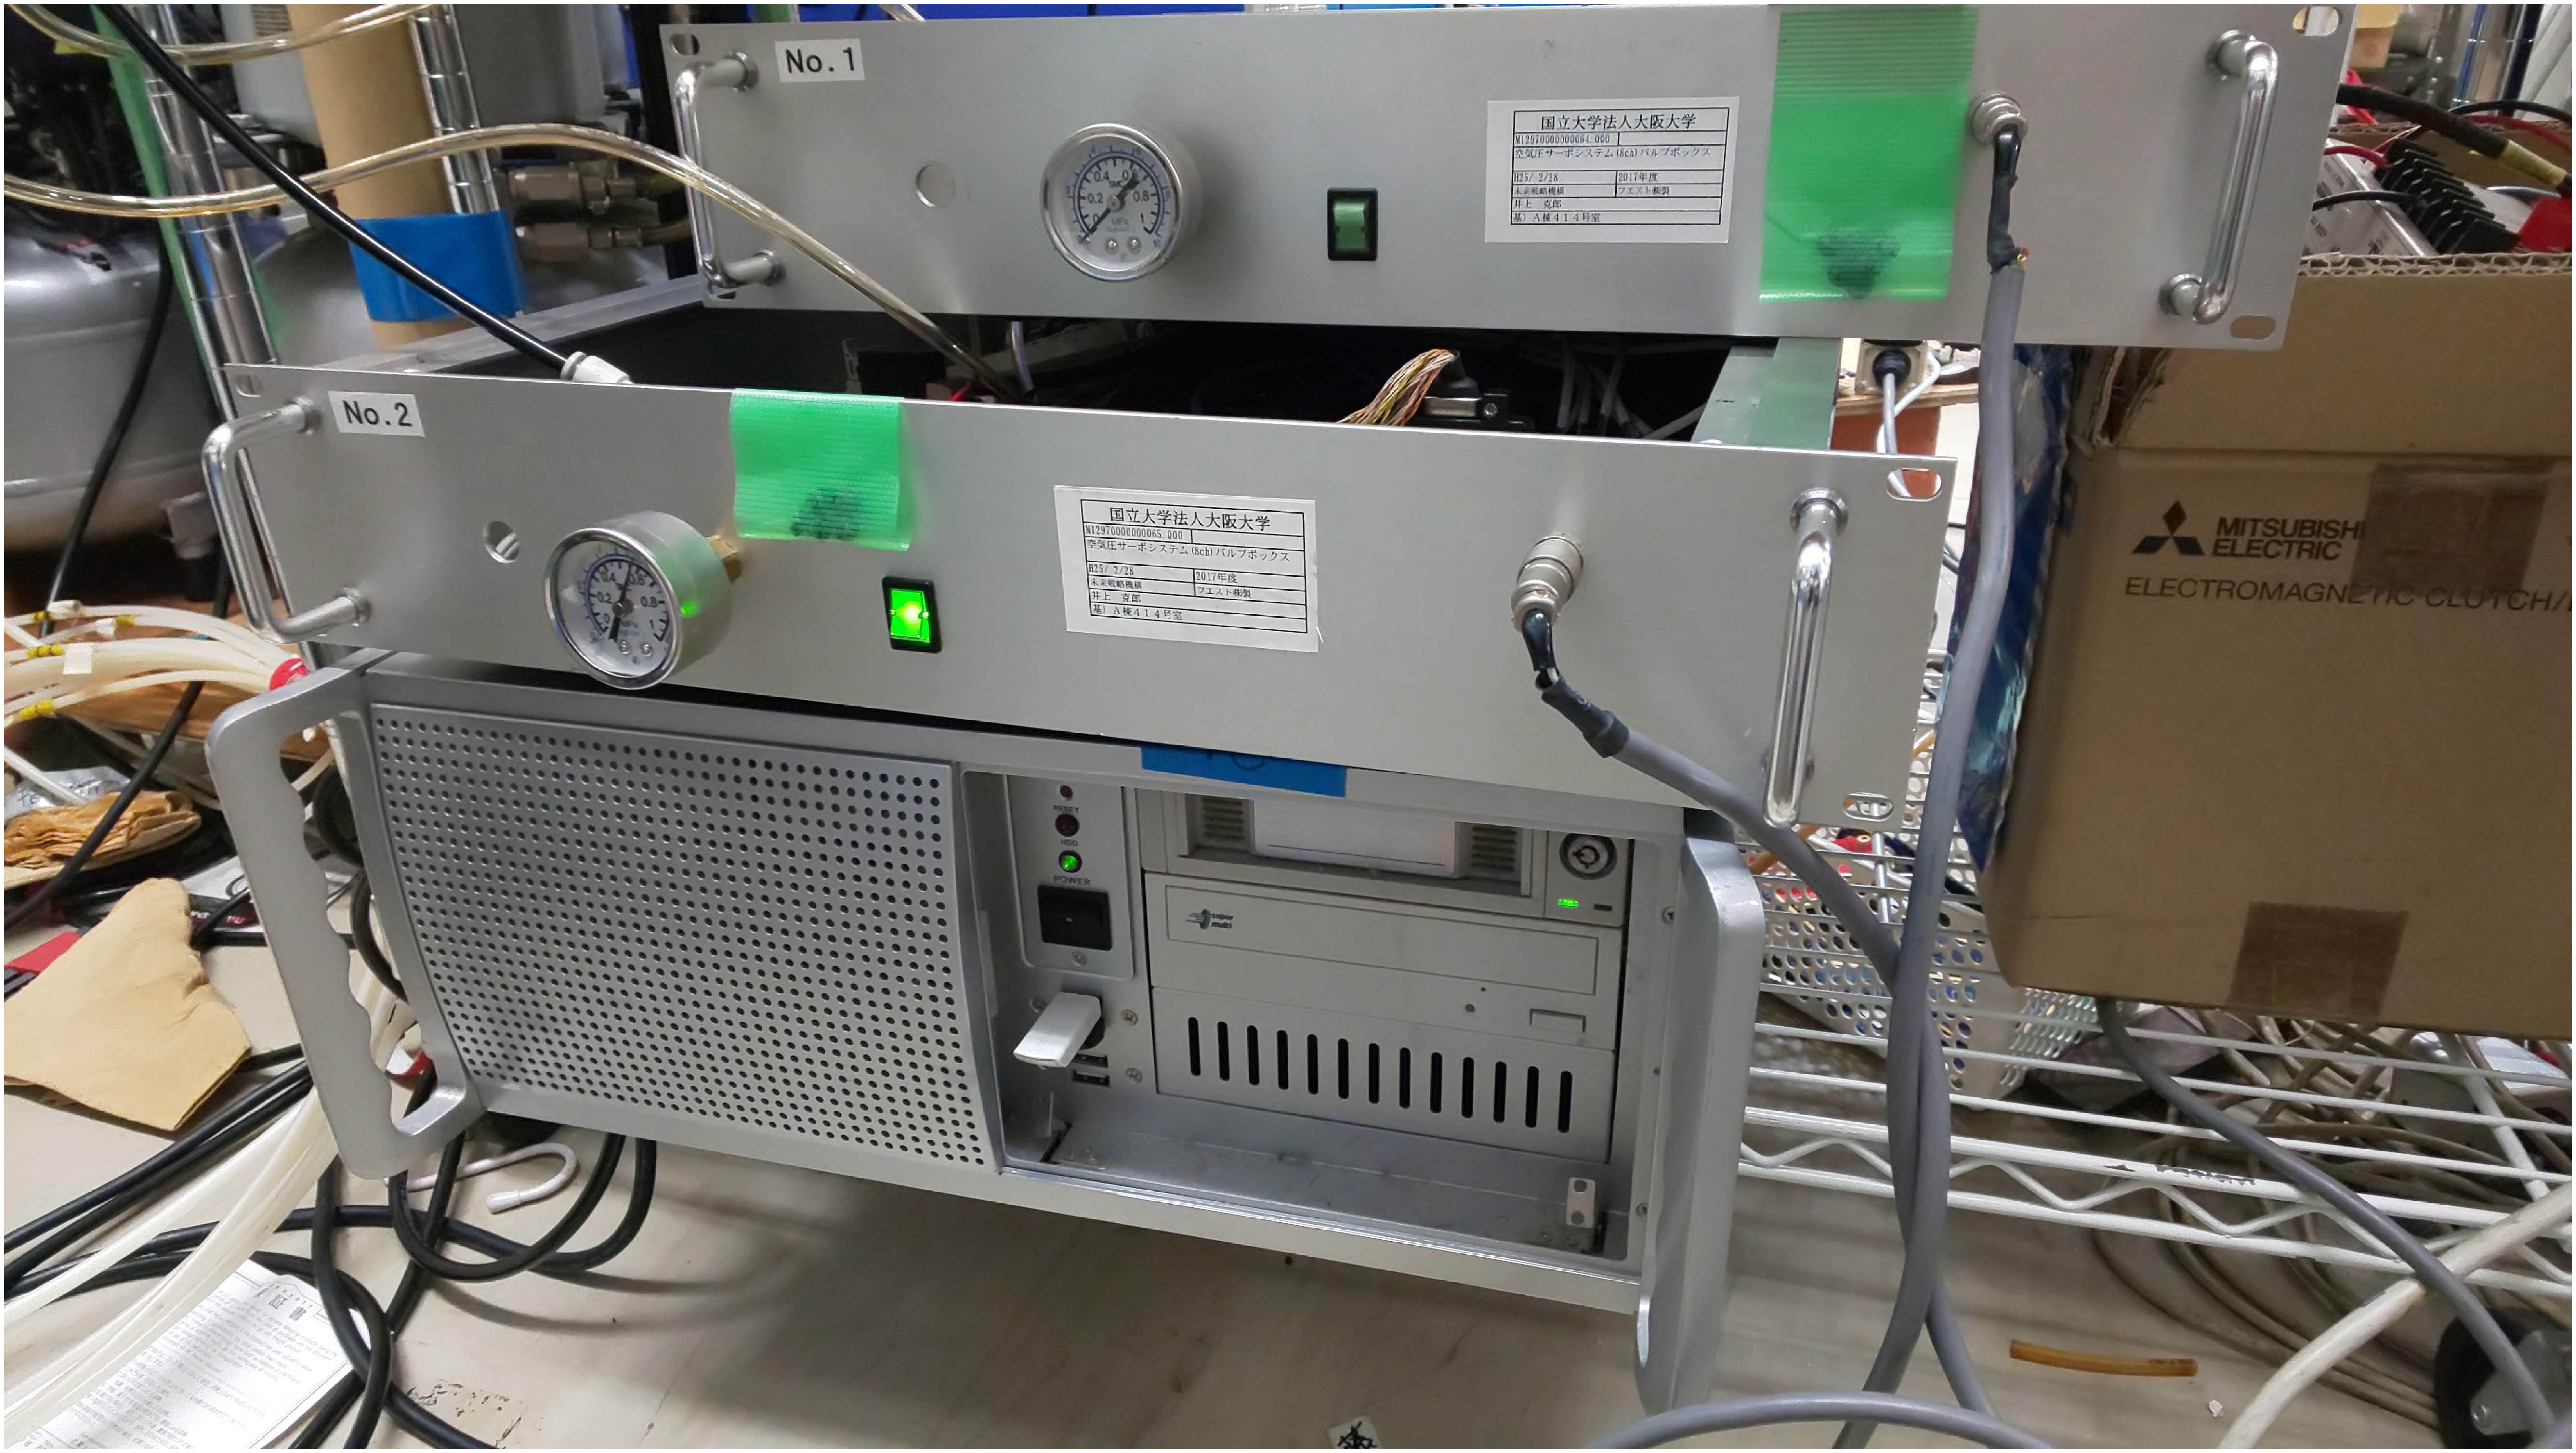
\includegraphics[width=0.65\columnwidth,clip]{./3_analysis/PC.eps}
     \caption{制御PCとエアー制御盤}
     \label{fig:PC}
    \end{center}
\end{figure}

\newpage

\section{実験手法}
\subsection{ストレッチセンサ計測精度評価}
今回製作した,ストレッチセンサの精度評価として各空気圧人工筋にsin出力を段階的に与えて,センサの計測値と,実際の長さの比較を行った.
実際の長さの計測は,ノギスを用いて計測を行った.与えた出力値は12段階とした.底背屈動作をモデルに検討を行うため,前脛骨筋と腓骨筋/ヒラメ筋の
組み合わせで出力を与えることとした.Fig.\ref{output_for_test}に示す様な出力を各空気圧人工筋に対して与えた.

センサでの時定数計測に関して,計測値を安定させるため30秒ほど記録を行った.
そしてその後,サンプル数$n$,計測値$t_i \left(i=0,1,\cdots,n\right)$としたとき,
\begin{eqnarray}
        \overline{t}=\frac{\sum_{i=0}^n t_i}{n}
        \label{ave}
\end{eqnarray}
といった式で求まる,総和平均$\overline{t}$を用いて時定数を求めた.
また,その誤差$\delta t$として,
\begin{eqnarray}
    \delta t = \sqrt{ \frac{\sum_{i=0}^n \left(t_i-\overline{t}\right)^2}{n(n-1)}}
    \label{std}
\end{eqnarray}
といった式で求まる,標準誤差を用いて計算した.

\begin{figure}[h]
    \begin{center}
        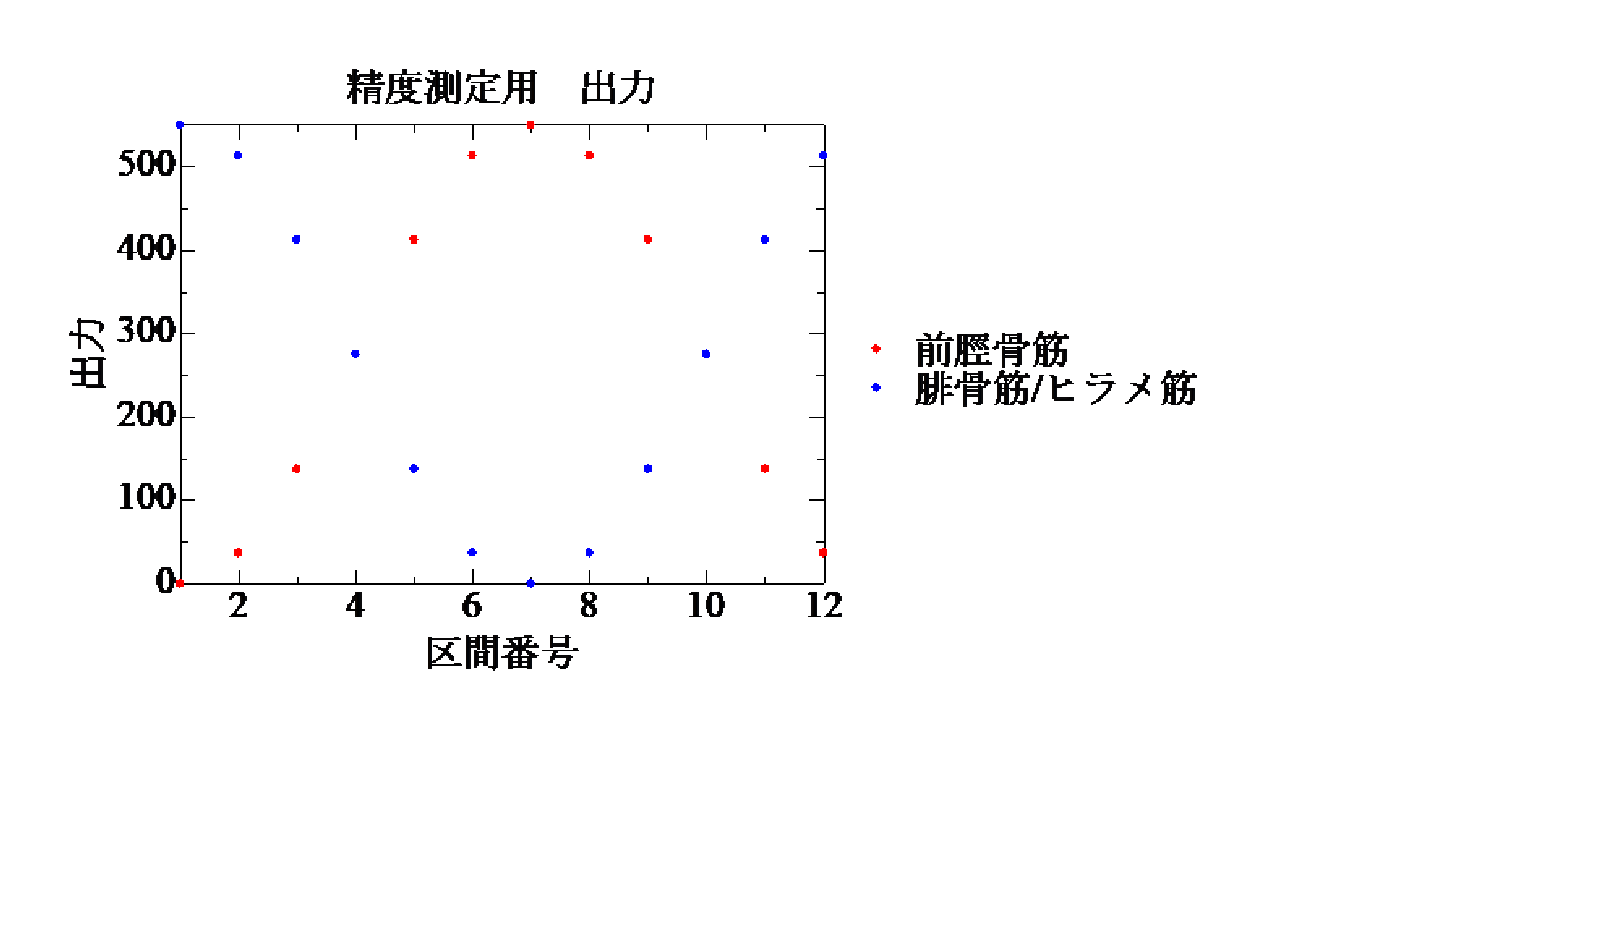
\includegraphics[width=0.76\columnwidth,clip]{2_measurement/output/output.eps}
        \caption{精度評価用 出力}
        \label{output_for_test}
    \end{center}
\end{figure}

\newpage

\subsection{ストレッチセンサ動的計測}
上記で計測した結果を元に、足関節ロボットに1Hzのsin周期運動をさせ、ストレッチセンサを用いて各筋の伸長計測を行った。
なお、各筋に与える出力はFig.\ref{output_for_actions}に示すものを与えた。

\begin{figure}[h]
  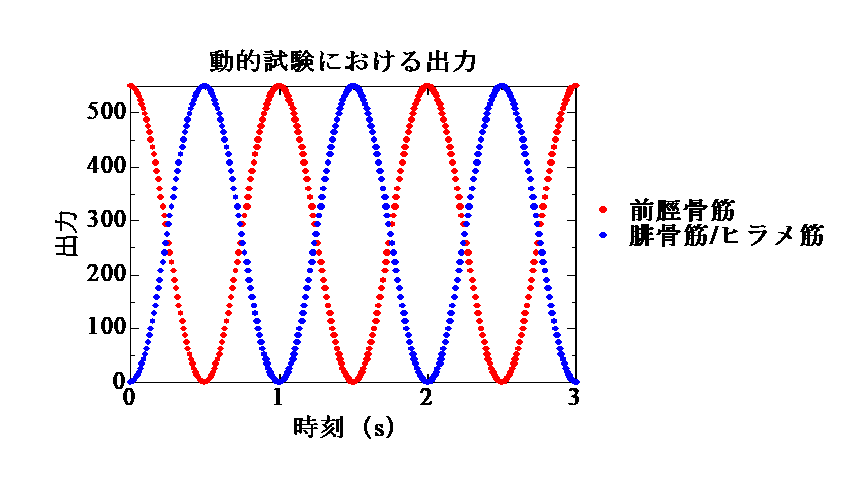
\includegraphics[width=0.76\columnwidth,clip]{3_analysis/outPut/putPut.eps}
  \caption{動的計測}
  \label{output_for_actions}
\end{figure}

解析方法として、与えた出力が1Hzであること、データの出力周期が100Hzであることを用いて、
1秒ごとに区切り0.01秒ごとの区間の平均値、標準誤差の計算を行った。
なお、それぞれの計算には式\ref{ave}、\ref{std}をそれぞれ用いた。
